\documentclass{standalone}
\usepackage[utf8]{inputenc}
\usepackage{tikz}
\begin{document}

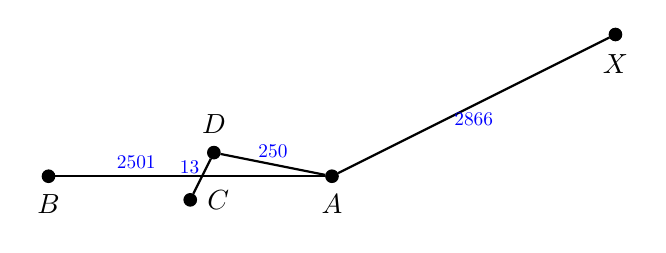
\begin{tikzpicture}[scale=.6]
% \draw[rounded corners=5mm, fill=gray!20, draw=white] (-.7,-.2) -- (3.5,0.7) -- (0.2,4.5) -- cycle;
%  \node[label={[gray]$T_{i_1/i}$}] (Ti1i) at (2,2) {}; 
  \begin{scope}[every node/.style={circle,draw=black,fill= black,minimum size=3.5pt, inner sep=1.6}];
  \node[label=below:$A$] (A) at (0,0) {};
  \node[label=below:$B$] (B) at (-6,0) {};
  \node[label=right:$C$] (C) at (-3,-0.5) {};
  \node[label=$D$] (D) at (-2.5,0.5) {};
  \node[label=below:$X$] (X) at (6,3) {};
  \end{scope}
	\draw[thick] (A) -- (B) node[pos=0.7, above, scale=0.7] {\textcolor{blue}{2501}}; 
	\draw[thick] (A) -- (X) node[pos=0.5, below, scale=0.7] {\textcolor{blue}{2866}};
	\draw[thick] (C) -- (D) node[pos=0.75,left, scale=0.7] {\textcolor{blue}{13}}; 
	\draw[thick] (D) -- (A) node[pos=0.5,above, scale=0.7] {\textcolor{blue}{250}};
  \end{tikzpicture}
  \end{document}
